% !TEX root = WaitFreeRingBuffer.tex

% !TEX root = WaitFreeRingBuffer.tex

\newcommand\fetchHead{
\begin{algorithm}[]
\caption{FetchHead $( )$ }
{\fontsize{8}{8}\selectfont
	\begin{algorithmic}[1]
		\State atomic\_fetch\_and\_increment(head)
	\end{algorithmic}
}
\label{alg:wf:example1}
\end{algorithm}
}

\newcommand\fetchTail{
\begin{algorithm}[]
\caption{FetchTail $( )$ }
{\fontsize{8}{8}\selectfont
	\begin{algorithmic}[1]
		\State atomic\_fetch\_and\_increment(tail)
	\end{algorithmic}
}
\label{alg:wf:example2}
\end{algorithm}
}

\newcommand\lfenqueue{
\begin{algorithm}[]
\caption{Enqueue $(val)$ }
{\fontsize{8}{8}\selectfont
	\begin{algorithmic}[1]
		\State TryHelpAnother()

		\State fail\_count = 0

		\While{true}
			\If {is\_full()} \label{alg:lf:enq:full}
				\State \Return false
			\EndIf

			\State seqid = next\_tail\_seq() \label{alg:enq:inc}
			\State pos = get\_position(seqid) \label{alg:enq:pos}
			\State  new\_node = new ElemNode(seqid, val) \label{alg:enq:elemnode}
			\While {true}
				\If {fail\_count++ $==$ MAX\_FAILS}
					\State op = new EnqueueOp(this, val)
					\State make\_announcement(op)
					\State \Return op.result()
				\EndIf

				\State node = buffer[pos].load()
				\If{node.op} \label{alg:enq:op}
					\State node.op.associate(node, \&(buffer[pos]))
					\State continue
				\ElsIf {isSkipped(node)} \label{alg:enq:bit}
					\State break
				\ElsIf {node.seqid $<$ seqid} \label{alg:enq:seqless}
					\State backoff()
					\If {node != buffer[pos].load()}
						\State continue
					\EndIf
				\EndIf

				\If {node.seqid $<=$ seqid  $and$ isEmpty(node)}
					\State success = buffer[pos].cas(node, new\_node) \label{alg:enq:common}
					\If {success}
						\State \Return true
					\EndIf
					\State continue
				\ElsIf {node.seqid $>$ seqid $or$ isElement(node)} \label{alg:enq:seqgreat}
					\State break
				\EndIf

			\EndWhile
		\EndWhile
	\end{algorithmic}
}
\label{alg:lf:enq}
\end{algorithm}
}

\newcommand\wfenqueue{
\begin{algorithm}[]
\caption{Wait-Free Enqueue $op$ }
{\fontsize{8}{8}\selectfont
	\begin{algorithmic}[1]
		\State seqid = get\_tail\_seq() -1
		\While{op.in\_progress()}
			\If {is\_full()}
				\State op.try\_set\_failed()
				\State \Return
			\EndIf

			\State seqid++
			\State pos = get\_position(seqid)
			\State  new\_node = new ElemNode(seqid, val, op)
			\While{op.in\_progress()}
				\State node = buffer[pos].load()
				\If{node.op}
					\State node.op.associate(node, \&(buffer[pos]))
					\State continue
				\ElsIf {isSkipped(node)}
					\State break
				\EndIf

				\If {node.seqid $<$ seqid}
					\State backoff()
					\If {node != buffer[pos].load()}
						\State continue
					\EndIf
				\EndIf

				\If {node.seqid $<=$ seqid  $and$ isEmpty(node)}
					\If {buffer[pos].cas(node, new\_node)}
						\State op.associate(new\_node, \&buffer[pos]);
						\State \Return
					\EndIf
				\ElsIf {node.seqid $>$ seqid $or$ isElement(node)}
					\State break
				\EndIf

			\EndWhile
		\EndWhile
	\end{algorithmic}
}
\label{alg:wf:enq}
\end{algorithm}
}


\newcommand\lfdequeue{
\begin{algorithm}[]
\caption{Dequeue $(\&result)$ }
{\fontsize{8}{8}\selectfont
	\begin{algorithmic}[1]
		\State TryHelpAnother()

		\State fail\_count = 0

		\While{true}
			\If {is\_empty()} \label{alg:lf:deq:empty}
				\State \Return false
			\EndIf

			\State seqid = next\_head\_seq() \label{alg:deq:inc}
			\State pos = get\_position(seqid) \label{alg:deq:pos}
			\State new\_node = new EmptyNode(seqid + capacity) \label{alg:deq:nullnode}
			\While{true}
				\If {fail\_count++ $==$ MAX\_FAILS} \label{alg:deq:maxfail}
					\State op = new DequeueOp(this)
					\State make\_announcement(op)
					\State \Return op.result(result)
				\EndIf

				\State node = buffer[pos].load()

				\If{node.op} \label{alg:deq:op}
					\State node.op.associate(node, \&(buffer[pos]))
					\State continue
				\ElsIf {isSkipped(node) $and$ isEmpty(node)} \label{alg:deq:fix}
					\If {buffer[pos].cas(node, new\_node)}
						\State break
					\Else
						\State continue
					\EndIf
				\ElsIf {seqid $ > $ node.seqid} \label{alg:deq:seqless}
					\State backoff()
					\If {node $==$ buffer[pos].load()}
						\If {isEmpty(node)}
							\If {buffer[pos].cas(node, new\_node)}
								\State break
							\EndIf
						\Else
							\State atomic\_mark\_skip(\&buffer[pos])
						\EndIf
					\EndIf
				\ElsIf {seqid $ < $ node.seqid} \label{alg:deq:seqgreat}
					\State break
				\Else % is not owned
					\If {isElem(node)}
						\If {isSkipped(node)}
							\State new\_node = setSkipped(new\_node)
						\EndIf
						\State success = buffer[pos].cas(node, new\_node) \label{alg:deq:common}
						\If {success}
							\State *result = node.value
							\State \Return true
						\EndIf
					\Else \label{alg:deq:nullnode}
					%isEmpty(node)
						\State backoff()
						\If {node $==$ buffer[pos].load()}
						 	\If {buffer[pos].cas(node, new\_node)}
								\State break
							\EndIf
						\EndIf
					\EndIf
				\EndIf

			\EndWhile
		\EndWhile
	\end{algorithmic}
}
\label{alg:lf:deq}
\end{algorithm}
}


\newcommand\wfdequeue{
\begin{algorithm}[]
\caption{Wait-Free Dequeue $(op)$ }
{\fontsize{8}{8}\selectfont
	\begin{algorithmic}[1]
		\State seqid = get\_head\_seq() -1
		\While{op.in\_progress()}
			\If {is\_empty()}
				\State \Return op.try\_set\_failed()
			\EndIf

			\State seqid++
			\State pos = get\_position(seqid)

			\While{op.in\_progress()}

				\State node = buffer[pos].load()

				\If{node.op}
					\State node.op.associate(node, \&(buffer[pos]))
					\State continue
				\ElsIf {isSkipped(node)}
					\If {isEmpty(node)}
						\If {buffer[pos].cas(node, new\_node) == false}
							\State continue
						\EndIf
					\EndIf
					\State break
				\Else %curr_node is not skip-marked
					\If {seqid $<$ node.seqid}
						\State backoff()
						\If {node $==$ buffer[pos].load()}
							\State break
						\EndIf
					\ElsIf {sec $>$ node.seqid}
						\State break
					\Else % seqid == node.seqid
						\If {isElem(node)}
							\State new\_node = new ElemNode(seqid, node.value, op)
							\If {buffer[pos].cas(node, new\_node)}
								\State op.associate(new\_node, \&(buffer[pos]))
								\State \Return
							\EndIf
						\Else
							\State break
						\EndIf
					\EndIf
				\EndIf
			\EndWhile
		\EndWhile
	\end{algorithmic}
}
\label{alg:wf:deq}
\end{algorithm}
}


\newcommand\dequeueassoc{
\begin{algorithm}[]
\caption{DequeueOp::associate $(node, address)$ }
{\fontsize{8}{8}\selectfont
\begin{algorithmic}[1]
	\State success = helper.cas(null, node) \label{alg:deq:assoc:lin}
	\If {success $or$ helper.load() == node}
		\State new\_node = NullNode(node.seqid + capacity)
		\If{address.cas(node,  new\_node) == false}
			\State node = setSkipped(node)
			\If{address.load() == node}
				\State new\_node = setSkipped(new\_node)
				\State address.cas(node,  new\_node)
			\EndIf
		\EndIf
	\Else
		\State node.op.store(null);
	\EndIf
\end{algorithmic}
}
\label{alg:deq:assoc}
\end{algorithm}
}

\newcommand\enqueueassoc{
\begin{algorithm}[]
\caption{EnqueueOp::associate $(node, address)$ }
{\fontsize{8}{8}\selectfont
\begin{algorithmic}[1]
	\State success = helper.cas(null, node)
	\If {success $or$ helper.load() == node}
		\State node.op.store(NULL)
	\Else
		\State new\_node = NullNode(node.seqid)
		\If{address.cas(node,  new\_node) == false}
			\State node = setSkipped(node)
			\If{address.load() == node}
				\State new\_node = setSkipped(new\_node)
				\State address.cas(node,  new\_node)
			\EndIf
		\EndIf
	\EndIf
\end{algorithmic}
}
\label{alg:enq:assoc}
\end{algorithm}
}
\newcommand\opTryFail{
\begin{algorithm}[]
\caption{Op::try\_set\_failed $()$ }
{\fontsize{8}{8}\selectfont
\begin{algorithmic}[1]
	\State helper.cas(null, FAIL) \label{alg:op:tryfail:lin}
\end{algorithmic}
}
\label{alg:op:tryfail}
\end{algorithm}
}

\newcommand\template{
\begin{algorithm}[]
\caption{template $(operand)$ }
{\fontsize{8}{8}\selectfont
\begin{algorithmic}[1]

\end{algorithmic}
}
\label{alg:template}
\end{algorithm}
}

%\lstset{
%  basicstyle=\small\singlespace,
%  morekeywords={const, atomic}
%}

In this section, we first present an overview of our approach, and then describe our specific implementation of the enqueue and dequeue operations.

In contrast to designs in which threads compete to finish an operation, our approach diffuses thread contention and reduces \SYN{forced dependency}.
We accomplish this through the use of sequence counters to \SYN{assign} order to threads performing enqueue and dequeue operations.
The presented implementation stores references \SYN{to} (\TY{of}) \descr{Node} objects in the ring buffer.
As described in Sec.~\ref{sec:definitions}, \descr{Node} objects contain a \emph{seqid} member, and if its is an \descr{ElemNode} it also contains an element member.
The position at which a \descr{Node} reference is placed, is determined by performing a mod operation on the \emph{seqid} using the length of the ring buffer.

Our implementation solves several dangers that may arise by using this methodology.
The first, is the case where an enqueue thread is assigned a position, but an \descr{ElemNode} already exists at that position.
The second, is the case where a dequeuer thread is assigned a position, but an \descr{EmptyNode}  exists at that position.
And a third danger, is the case where a dequeuer thread is assigned a position that holds a value, but its \emph{seqid} is less than the thread's \emph{seqid}.
These dangers can arise as a result of poor system scheduling, \SYN{inopportune} context switches, and thread delay. % @Steven, the examples are different but seem similar and redundant IMO
Our implementations include a novel solution that uses the atomic fetch and or (\op{fao}) operation along with the \emph{seqid} to ensure that these dangers do not affect the correctness of our implementation.


The remainder of this section is structured as follows:
We present a detailed explanation of enqueue and dequeue operations.
This explanation includes algorithm \SYN{behavior}, linearizability, and wait-freedom descriptions.
Next, provide several case examples using Figs.~\ref{todo} to describe several execution scenarios.
\SYN{After which}, we present an informal reasoning on algorithm correctness and linearizability.


\begin{figure*}[ht!]
\centering
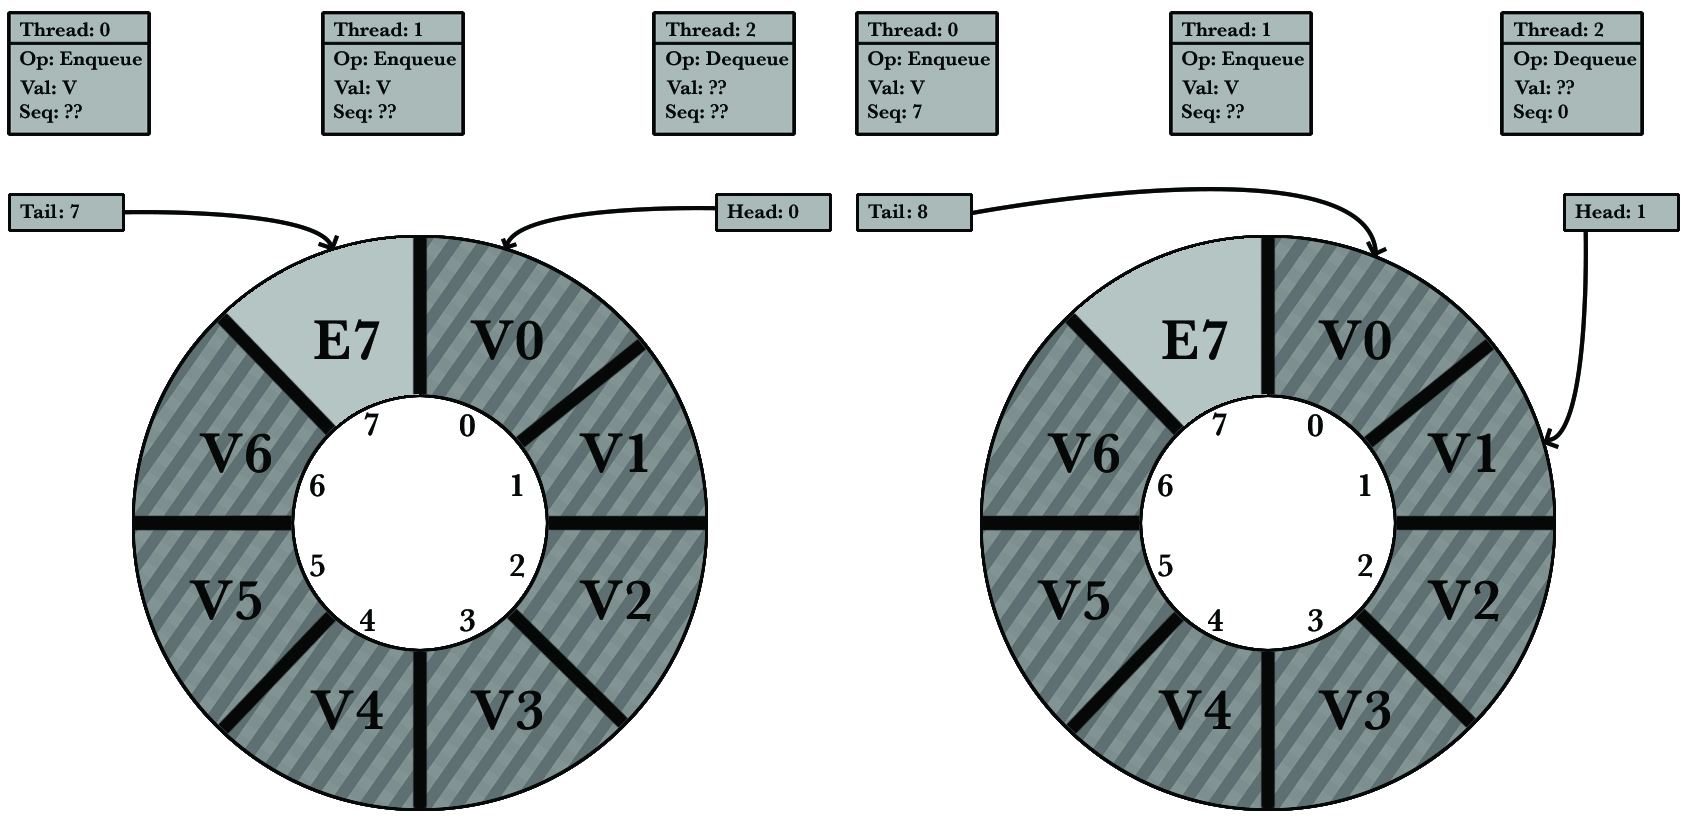
\includegraphics[width=90mm]{figures/buffer_init.jpg}
\caption{Init}
\label{buffer_ex}
\end{figure*}

\begin{figure}[ht!]
\centering
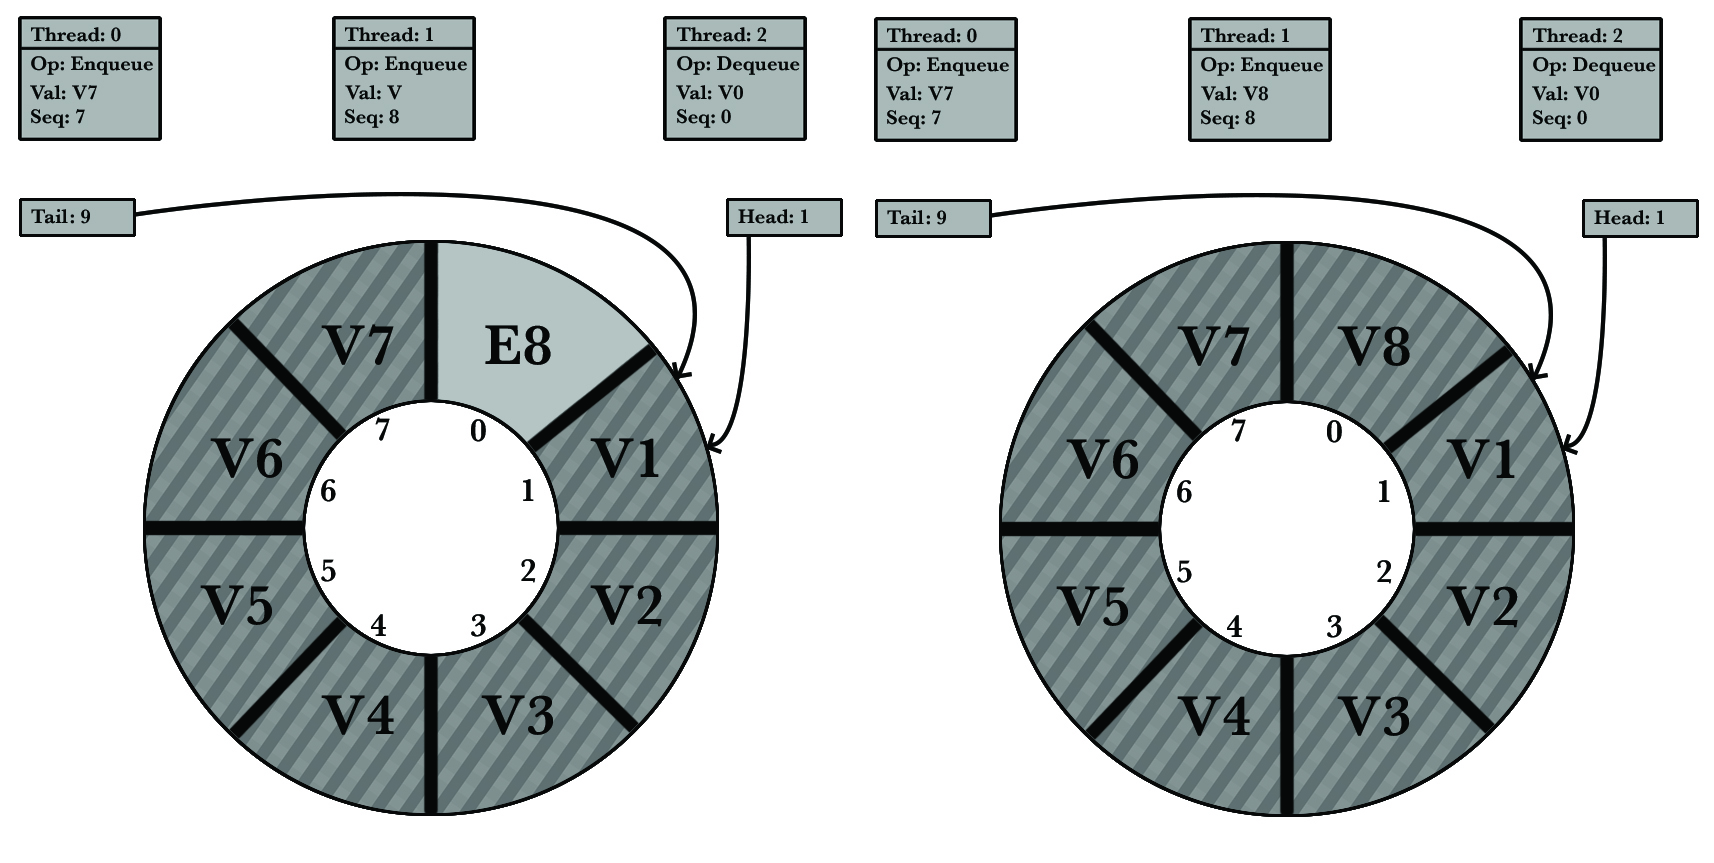
\includegraphics[width=90mm]{figures/buffer_ideal.jpg}
\caption{Ideal}
\label{buffer_ex}
\end{figure}

\begin{figure}[ht!]
\centering
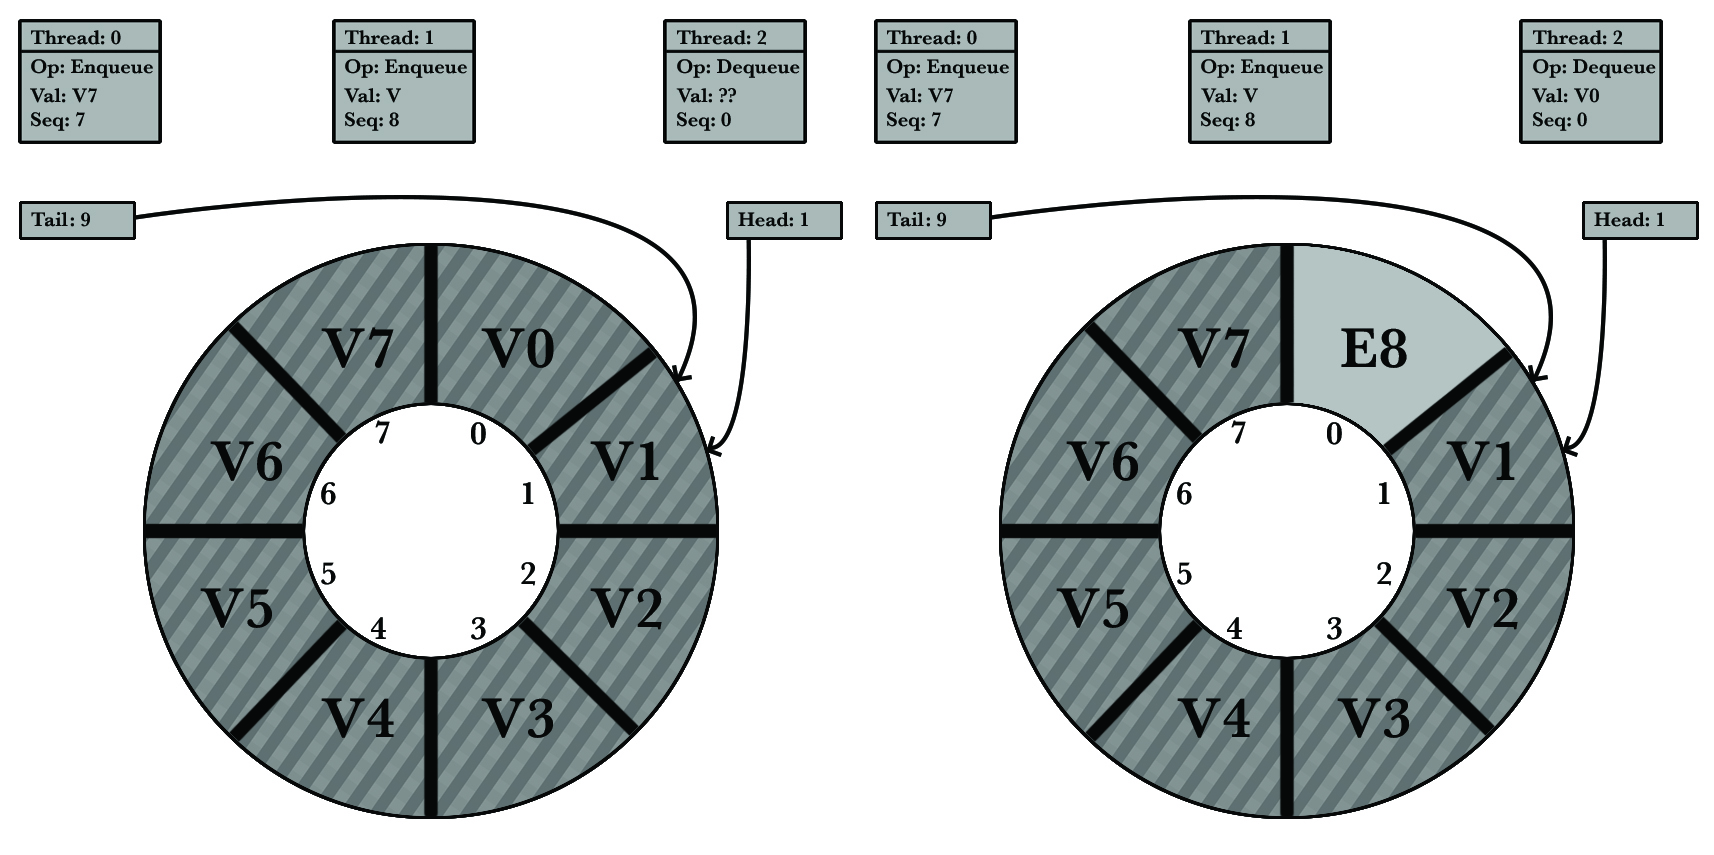
\includegraphics[width=90mm]{figures/buffer_full.jpg}
\caption{Full}
\label{buffer_ex}
\end{figure}


% ==============================
\section{Dequeue} % =========
\label{sec:alg:deq}
% ==============================

% =~=~=~=~=~=~=~=~=~=~=~=~=~=~=~
\lfdequeue % =~=~=~=~=~=~=~=~=~=
\wfdequeue % =~=~=~=~=~=~=~=~=~=
\opTryFail
\dequeueassoc % =~=~=~=~=~=~=~=~=~=


The following describes how a dequeue operation is performed. % @Steven, shouldnt this be implied enough by the section header and if not it seems a bit blunt
To guide the reader, we reference specific lines in Alg.~\ref{alg:lf:deq}

To \op{dequeue} an element, a thread will first check if the ring buffer is empty (L.~\ref{alg:lf:deq:empty}), returning false if it is.
Otherwise, it will acquire a dequeue sequence number, \emph{seqid}, from the head counter and determine the position, \emph{pos}, to dequeue an element (L.~\ref{alg:deq:inc}-~\ref{alg:deq:pos}).
The thread will then prepare an \descr{EmptyNode} to replace the dequeued value (L.~\ref{alg:deq:EmptyNode}). % @Steven, are we going back this route? you told me before to change the code to be as local with its usage as possible with the EmptyNode preaparation
The \emph{seqid} of the \descr{EmptyNode} is set to the assigned \emph{seqid} plus the buffer's capacity.
In the common case,  the thread will replace an \descr{ElemNode}, whose \emph{seqid} matches its assigned \emph{seqid}, with the prepared \descr{EmptyNode} (L.~\ref{alg:deq:common}).
Uncommon cases, which are often the result of thread delay, are described below.


\begin{itemize}
\item The node holds a reference to an operation record (L.~\ref{alg:deq:op}).
This indicates the node was placed as part of another thread's operation.
The thread will call the associate function for that operation and upon its return either the node has been replaced or the reference to the operation record has been removed.
The node at the current position will then be re-examined.

\item The node currently at the position has a \emph{seqid} number less than the assigned or it is an \descr{EmptyNode} \emph{seqid}(L.~\ref{alg:deq:seqless}, L.~\ref{alg:deq:EmptyNode}).
In this event, we call the backoff routine to provide an opportunity for a delayed thread to complete its operation.
If the current node has not changed the thread will advance the position by either replacing an \descr{EmptyNode} with the prepared \descr{EmptyNode} or performing an atomic bitmark if it is an \descr{ElemNode}.
If the node has changed, the position will be re-examined.

In order to achieve FIFO ordering, threads can only remove an \descr{ElemNode} if it was assigned that node's \emph{seqid}.
The atomic bitmark allows a thread to get a new \emph{seqid} without the risk of an \descr{ElemNode} being enqueued with a \emph{seqid} that has been given up. % @Steven, we should work to make this more clear when we revise together

\item The node currently at the position is bitmarked and an \descr{EmptyNode} (L.~\ref{alg:deq:fix}).
This state resulted from the previously described, in which a thread bitmarked an \descr{ElemNode}.
The thread who was assigned that node's \emph{seqid} must have replaced it with a bitmarked \descr{EmptyNode}.
Sec.~\ref{sec:correctness} describes the importance of replacing a bitmarked \descr{ElemNode} with a bitmarked \descr{EmptyNode}.
This state is resolved by replacing  the bitmarked \descr{EmptyNode} with  an unbitmarked \descr{EmptyNode}.

\item The node currently at the position has a \emph{seqid} greater than the assigned \emph{seqid} (L.~\ref{alg:deq:seqgreat}).
This implies that some thread caused this thread's \emph{seqid} to be skipped and as result this thread needs to get a new \emph{seqid}.

\end{itemize}

% @Steven, I feel the new code is well described but the flow and structure of the code itself makes it more difficult to follow. I also think with the progress assurance that follows this, I think it gives the impression the code heavily relies on the progress assurance to achieve wait-freedom rather than in the last structure it seemed easier to see the rarity. But after reading enqueue Ive slightly changed my mind

These uncommon cases could force a thread to indefinitely reattempt its operation.
However, we employ a progress assurance scheme to prevent this from occurring.
Specifically, in the event a threshold is reached (L.~\ref{alg:deq:maxfail}) the thread will make an announcement and switch to a slow path dequeue operation (Alg.~\ref{alg:wf:deq}). We describe in Sec.~\ref{sec:progressassurance}, specifically how this announcement scheme is used to ensure an operation is completed in a finite number of steps.

The wait-free dequeue operation functions very similarly to the normal dequeue operation with the following key change.
\begin{itemize}
\item The operation ends when some threads calls either \emph{op.try\_set\_failed} or \emph{op.associate}.
Upon return of these functions it is guaranteed that the operation has been completed.
\item The thread is not assigned a \emph{seqid} but instead loads the current value of the head counter.
This is important to prevent the scenario where a thread is assigned a position after the operation has been completed and as a result no longer needs to dequeue a value.
\item The node placed holds a reference to the operation record it was placed on behalf of.
This is used to prevent the case where multiple threads complete the same operation.
Multiple nodes may reference the same operation record, but the operation record may only refence one of these nodes: the completed operation.
\item After a node is placed, the operation's associate function is called.
This ensures that if the node was placed incorrectly its reference to the operation record will be removed.
If it was placed correctly, then the node will be replaced by an \descr{EmptyNode}.

\end{itemize}


\subsection{Linearizability}
In general the linearization point for a successful dequeue operation is the atomic \op{faa} operation which assigned the \emph{seqid} (L.~\ref{alg:deq:inc}).
However, this is not realized until the thread successfully places an \descr{EmptyNode} in place of the \descr{ElemNode} with \emph{seqid} matching the \emph{seqid} assigned (L.~\ref{alg:deq:common}).
If the wait-free path is used then the linearization point for a successful dequeue operation is the successful association of an \descr{ElemNode} and a \descr{DequeueOp} (Alg.~\ref{alg:deq:assoc} L.~\ref{alg:deq:assoc:lin}).

The linearization point for a failed dequeue operation is when a thread thread detects that the ring buffer is empty  (Alg.~\ref{alg:lf:deq} L.~\ref{alg:lf:deq:empty}).

If the wait-free path is used then the linearization point for a failed dequeue operation is the successful \op{cas} that set the operation's \emph{helper} member to the \emph{FAIL} constant (Alg.~\ref{alg:op:tryfail} L.~\ref{alg:op:tryfail:lin}).


% ==============================
\section{Enqueue} % =========
\label{sec:alg:dequeue}
% ==============================

% =~=~=~=~=~=~=~=~=~=~=~=~=~=~=~
\lfenqueue % =~=~=~=~=~=~=~=~=~=
\wfenqueue % =~=~=~=~=~=~=~=~=~=
\enqueueassoc % =~=~=~=~=~=~=~=~=~=
% =~=~=~=~=~=~=~=~=~=~=~=~=~=~=~

The following describes how a enqueue operation is performed.
To guide the reader, we reference specific lines in Alg.~\ref{alg:lf:enq}

To \op{enqueue} an element, a thread will first check if the ring buffer is full (L.~\ref{alg:lf:enq:full}), returning false if it is.
Otherwise, it will acquire a enqueue sequence number, \emph{seqid}, from the tail counter and determine the position, \emph{pos}, to enqueue an element (L.~\ref{alg:enq:inc}-~\ref{alg:enq:pos}).
The thread will then prepare an \descr{ElemNode} to hold the element being enqueued (L.~\ref{alg:enq:elemnode}).
The \emph{seqid} of the \descr{ElemNode} is set to the assigned \emph{seqid}.
In the common case,  the thread will replace an \descr{EmptyNode}, whose \emph{seqid} matches its assigned \emph{seqid}, with the prepared \descr{ElemNode} (L.~\ref{alg:enq:common}).
Uncommon cases, which are often the result of thread delay, are described below.

\begin{itemize}
\item The node holds a reference to an operation record (L.~\ref{alg:enq:op}).
This indicates the node was placed as part of another thread's operation.
This must be resolved by calling the associate function for that operation.
Upon its return either the node has been replaced or the reference to the operation record has been removed.
The thread will then re-examine the current position.

\item The reference currently at the position has a bitmark (L.~\ref{alg:enq:bit}), indicating it was marked as skipped.
This indicates the node at the position needs to be fixed by a dequeue thread.
As a result, the enqueue thread will get a new \emph{seqid} and retry its operations.

\item The node currently at the position has a \emph{seqid} number less than the assigned the \emph{seqid} (L.~\ref{alg:enq:seqless}).
In this event,the thread will call the backoff routine to provide time for a delayed thread to complete its operation.
If the current node has not changed and it is an \descr{EmptyNode} the thread will attempt to replace it with the prepared \descr{ElemNode}.
Otherwise, it will get a new \emph{seqid}.

\item The node currently at the position has a \emph{seqid} greater than the assigned \emph{seqid} (L.~\ref{alg:enq:seqgreat}).
This implies that some thread caused this thread's \emph{seqid} to be skipped and as result this thread needs to get a new \emph{seqid}.

\end{itemize}

As described in Sec.~\ref{sec:alg:dequeue}, these uncommon cases could force a thread to indefinitely reattempt its operation.
The following are key differences between the normal enqueue operation and the wait-free enqueue operation.
\begin{itemize}
\item The operation ends when some threads calls either \emph{op.try\_set\_failed} or \emph{op.associate}. % line 4, 13, 26
Upon return of these functions it is guaranteed that the operation has been completed.
\item The thread is not assigned a \emph{seqid} but instead loads the current value of the tail counter.
This is important for achieving maximum unskipped buffer indices resulting from cancelled operations.
%This is important to prevent the scenario where a thread is assigned a position after the operation has been completed and as a result no longer needs to enqueue a value.
\item The node placed holds a reference to the operation record it was placed on behalf of.
This is used to prevent the case where multiple threads complete the same operation.
Many nodes may reference the same operation record, but the operation record may only refence one of these nodes: the completed operation.
\item After a node is placed, the operation's associate function is called.
This ensures that if the node was placed incorrectly then the node will be replaced by an \descr{EmptyNode}.
If it was placed correctly, its reference to the operation record will be removed.

\end{itemize}

\section{Wait-Freedom}
We show that both the dequeue and enqueue algorithms are wait-free by first examining the loops and their terminating conditions. Both algorithms contain two nested while loops and in general the outer loop executes until the operation has been completed and the inner loop executes until the assigned \emph{seqid} is no longer viable.
The \emph{MAX\_FAILS} constant is used to place an upper bound on the number of times a thread will execute these loops.
If this constant is reached, \op{make\_announcement} is called and be our definition of this function upon its return the operation must be complete. Thus if all functions called by \op{dequeue} or \op{enqueue}, then these functions are wait-free.


Except for  \op{TryHelpAnother} and \op{make\_announcement}, the functions called are utility functions that are used to simplify the code explanation.
These functions are inherently wait-free because they contain no loops or calls to non-wait-free functions.
However, both \op{TryHelpAnother} and \op{make\_announcement} are capable of calling \op{wait-free dequeue} or \op{wait-free enqueue}, thus wait-freedom is determined by the progress guarantee of these two operations.

Both \op{wait-free dequeue} or \op{wait-free enqueue} employ the same looping structures which terminate when the operation record (\emph{op}) is no longer in progress. An operation record is in progress as long as its \emph{helper} member is \emph{null}.
\TODO{discuss how its lf and blah blah and if it enough operations occur, all threads will be helping, thus it is wait-free...}
